% \documentclass[xcolor=dvipsnames]{beamer}
% \usepackage{beamerthemesplit}
% \usepackage{bm,amsmath,color}
% \definecolor{darkblue}{rgb}{0.0,0.0,0.50}
% \definecolor{myorange}{cmyk}{0,0.7,1,0}
% \hypersetup{colorlinks = true, linkcolor=darkblue, citecolor=darkblue, 
% urlcolor=darkblue}
% \hypersetup{pdfauthor={Samwise the great}, pdftitle={Really it is a tale of samwise}}
% 
% %% create a color to highlight things
% \newcommand{\highlt}{\textcolor {myorange}}
% 
% %% set beamer theme and color change them as you want
% \usetheme{Frankfurt}
% \usecolortheme{rose}
% \setbeamertemplate{blocks}[rounded][shadow=true]

%% beamer packages
% other themes: AnnArbor, Antibes, Bergen, Berkeley, Berlin, Boadilla, boxes, 
% CambridgeUS, Darmstadt, Dresden, Frankfurt, Goettingen, Hannover, Ilmenau,
%JuanLesPins, Luebeck, Madrid, Malmoe, Marburg, Montpellier, PaloAlto,
%Pittsburgh, Rochester, Singapore, Szeged, Warsaw
% other colors: albatross, beaver, crane, default, dolphin, dove, fly, lily, 
%orchid, rose, seagull, seahorse, sidebartab, structure, whale, wolverine,
%beetle

\documentclass[xcolor=dvipsnames]{beamer}
\usepackage{beamerthemesplit}
\usepackage{bm,amsmath,marvosym}
\usepackage{listings,color}%xcolor
\usepackage[utf8]{inputenc}
\definecolor{shadecolor}{rgb}{.9, .9, .9}
\definecolor{darkblue}{rgb}{0.0,0.0,0.5}
\definecolor{myorange}{cmyk}{0,0.7,1,0}
\definecolor{mypurple}{cmyk}{0.3, 0.9, 0.0, 0.2}

\lstnewenvironment{code}{
    \lstset{backgroundcolor=\color{shadecolor},
        showstringspaces=false,
        language=python,
        frame=single,
        framerule=0pt,
        keepspaces=true,
        breaklines=true,
        basicstyle=\ttfamily,
        keywordstyle=\bfseries,
        basicstyle=\ttfamily\scriptsize,
        keywordstyle=\color{blue}\ttfamily,
        stringstyle=\color{red}\ttfamily,
        commentstyle=\color{green}\ttfamily,
        columns=fullflexible
    }
}{}

\lstnewenvironment{codeout}{
    \lstset{backgroundcolor=\color{shadecolor},
        frame=single,
        framerule=0pt,
        breaklines=true,
        basicstyle=\ttfamily\scriptsize,
        columns=fullflexible
    }
}{}

\hypersetup{colorlinks = true, linkcolor=darkblue, citecolor=darkblue,urlcolor=darkblue}
\hypersetup{pdfauthor={A. Richards}, pdftitle={a tale of a hobbits tale}}

\newcommand{\rd}{\textcolor{red}}
\newcommand{\grn}{\textcolor{green}}
\newcommand{\highlt}{\textcolor{myorange}}
\newcommand{\norm}[1]{\left\lVert#1\right\rVert}
\def\ci{\perp\!\!\!\perp}

% set beamer theme and color
\usetheme{Frankfurt}
%\usetheme{Boadilla}
%\usecolortheme{dolphin}
\usecolortheme{seagull}
%\setbeamertemplate{blocks}[rounded][shadow=true]

\title[plotting]{Basic Plotting}
\author[AJR]{Adam Richards}
\institute{Galvanize, Inc}
\date[\today]{Last updated: \today}

%%%%%%%%%%%%%%%%%%%%%%%%%%%%%%%%%%%%%%%%%%%%%%%%%%%%%%%%%%%%%%%%%%%%%%%%%%%%%%%
\begin{document}
\frame{\titlepage}
%%%%%%%%%%%%%%%%%%%%%%%%%%%%%%%%%%%%%%%%%%%%%%%%%%%%%%%%%%%%%%%%%%%%%%%%%%%%%%%
\frame{
\footnotesize
\tableofcontents
\normalsize
}

%%%%%%%%%%%%%%%%%%%%%%%%%%%%%%%%%%%%%%%%%%%%%%%%%%%%%%%%%%%%%%%%%%%%%%%%%%%%%%%
\frame{
\begin{block}{Goals}
\begin{enumerate}
 \item Understand how figures, subplots, axes work together in matplotlib, seaborn, and pandas
 \item Use plots and subplots effectively to explore a dataset
 \item Distinguish between different categories on the same plot
 \item Plot inside and outside of ipython notebooks
 \item Understand MPL fundamentals well enough to learn effectively
\end{enumerate}
 \end{block}

\ \\ 
For the morning, we will go through a gentle introduction to Matplotlib setting the stage for the afternoon assignment.
The goal for this morning is to get more practice with EDA and Pandas.
 
}

%%%%%%%%%%%%%%%%%%%%%%%%%%%%%%%%%%%%%%%%%%%%%%%%%%%%%%%%%%%%%%%%%%%%%%%%%%%%%%%
\section{matplotlib}
\subsection{}
%%%%%%%%%%%%%%%%%%%%%%%%%%%%%%%%%%%%%%%%%%%%%%%%%%%%%%%%%%%%%%%%%%%%%%%%%%%%%%%

%%%%%%%%%%%%%%%%%%%%%%%%%%%%%%%%%%%%%%%%%%%%%%%%%%%%%%%%%%%%%%%%%%%%%%%%%%%%%%%
\frame{
\frametitle{matplotlib}
\footnotesize
\begin{block}{}
The most frequently used plotting package in Python, \href{http://matplotlib.org}{matplotlib}, is written in pure Python and is heavily dependent on \href{http://www.numpy.org}{NumPy}. 
\end{block}

\begin{columns}
 
 \begin{column}{7.5cm}
 \begin{itemize}
  \item Plots should look great i.e. publication quality
  \item Text should look great (antialiased, etc.)
  \item Postscript output for inclusion with \TeX\ documents
  \item Embeddable in a GUI for application development
  \item Code should be easy to understand and extend
  \item Making plots should be easy 
 \end{itemize}
 \end{column}

 \begin{column}{2.5cm}
   \begin{center}
  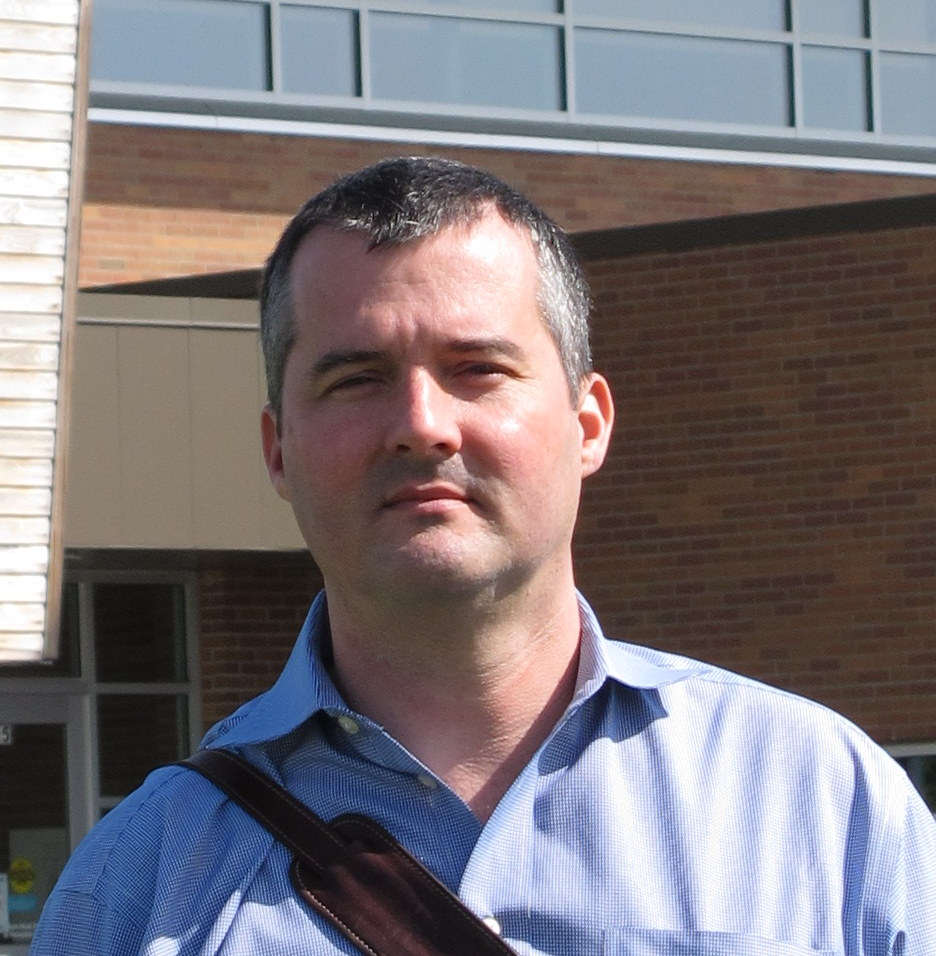
\includegraphics[scale=0.08]{john-hunter.jpg}
 \end{center}
 \end{column}

\end{columns}

\begin{flushleft}
 When using in publications or white papers $\rightarrow$ \cite{Hunter07}
\end{flushleft}  
}

%%%%%%%%%%%%%%%%%%%%%%%%%%%%%%%%%%%%%%%%%%%%%%%%%%%%%%%%%%%%%%%%%%%%%%%%%%%%%%%%
\begin{frame}[fragile]
\scriptsize

Matplotlib is conceptually divided into three parts:

\begin{itemize}
 \item \highlt{pylab} interface (similar to MATLAB) - \href{http://matplotlib.org/users/pyplot_tutorial.html#pyplot-tutorial}{pylab tutorial}
 \item \highlt{Matplotlib frontend} or API - \href{http://matplotlib.org/users/artists.html#artist-tutorial}{artist tutorial}
 \item \highlt{backends} - drawing devices or renderers 
\end{itemize}

\begin{columns}
 \begin{column}{5cm}
  \begin{code}
import matplotlib.pyplot as plt
plt.plot([1,2,3,4])
plt.ylabel('some numbers')
plt.show()
  \end{code}
 \end{column}
 \begin{column}{5cm}
\begin{code}
import matplotlib.pyplot as plt
fig = plt.figure()
ax = fig.add_subplot(1,1,1)
ax.set_ylabel('some numbers')
ax.plot([1,2,3,4])
plt.show()
  \end{code}
 \end{column}
\end{columns}

\begin{center}
  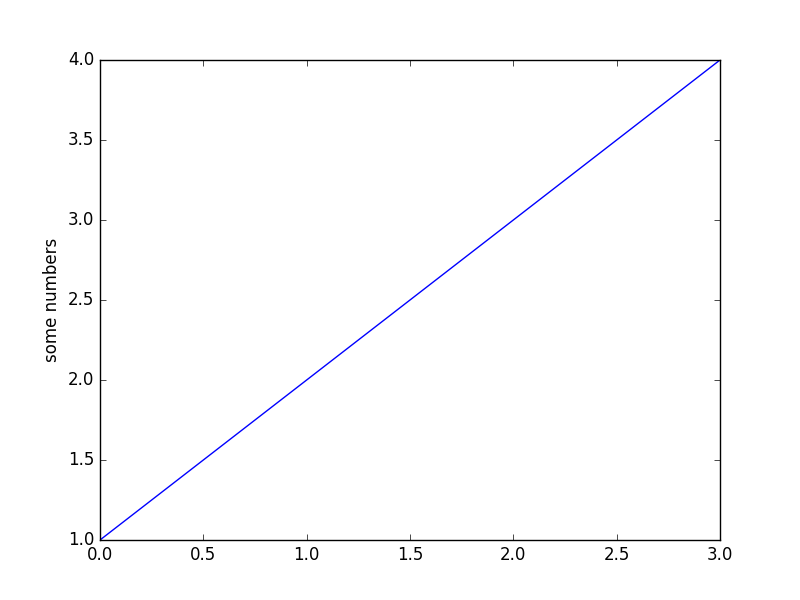
\includegraphics[scale=0.2]{simple.png}
\end{center}
\begin{flushleft}
 \tiny{Note that the x-axis was automatically generated} 
\end{flushleft}
\end{frame}

%%%%%%%%%%%%%%%%%%%%%%%%%%%%%%%%%%%%%%%%%%%%%%%%%%%%%%%%%%%%%%%%%%%%%%%%%%%%%%%
\frame{
\frametitle{On Jupyter and data visualization...}
\scriptsize
\begin{block}{}
 Who is in your audience?
\end{block}

\begin{itemize}
 \item How much customization do I need?
 \item How fast does it need to be done?
 \item Is it complicated?
 \item Version control, reproducibility
\end{itemize}

So many choices...
\begin{enumerate}
 \item \highlt{Environment} - IPython, Jupyter, scripts, Sphinx, reportlab 
 \item \highlt{Plotting tool} - Pandas, Seaborn, Plotly, Bokeh, MPL-pylab, MPL-artist
 \item \highlt{Deliverable} - webpage, report, presentation, white-paper, publication, dashboard
\end{enumerate}
  
\begin{block}{}
 What is it that is I \highlt{expect} to see?
\end{block}
}

%%%%%%%%%%%%%%%%%%%%%%%%%%%%%%%%%%%%%%%%%%%%%%%%%%%%%%%%%%%%%%%%%%%%%%%%%%%%%%%%
\frame{
\frametitle{It can get complicated...}
\begin{center}
  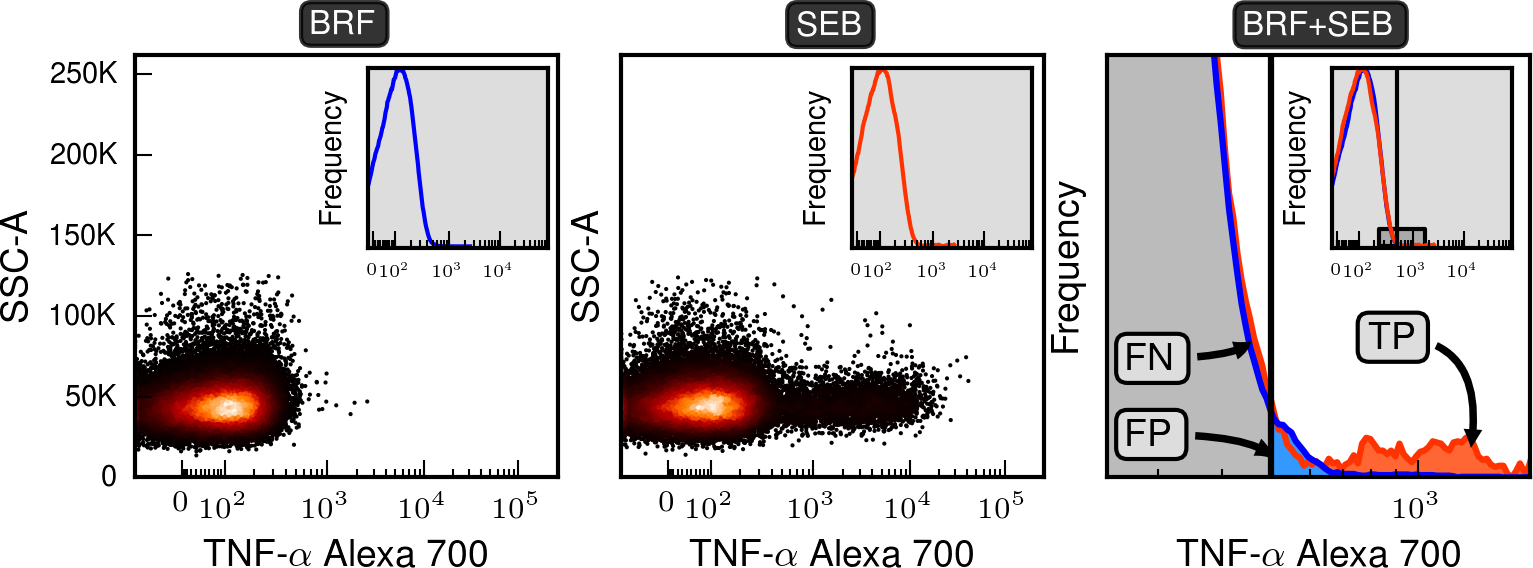
\includegraphics[scale=0.7]{complicated.png}
\end{center}

\begin{flushleft}
  \tiny{\href{http://www.sciencedirect.com/science/article/pii/S0022175914001185}{http://www.sciencedirect.com/science/article/pii/S0022175914001185}}
\end{flushleft}
}

%%%%%%%%%%%%%%%%%%%%%%%%%%%%%%%%%%%%%%%%%%%%%%%%%%%%%%%%%%%%%%%%%%%%%%%%%%%%%%%
\section{plotting}
\subsection{}
%%%%%%%%%%%%%%%%%%%%%%%%%%%%%%%%%%%%%%%%%%%%%%%%%%%%%%%%%%%%%%%%%%%%%%%%%%%%%%%%

%%%%%%%%%%%%%%%%%%%%%%%%%%%%%%%%%%%%%%%%%%%%%%%%%%%%%%%%%%%%%%%%%%%%%%%%%%%%%%%%
\begin{frame}[fragile]
\frametitle{mpl basics}
\scriptsize
\begin{columns}
\begin{column}{5cm}
The shell...
 \begin{code}
  import matplotlib.pyplot as plt
  plt.figure(figsize=(8,6))
  ax = plt.add_subplot(1,1,1)
  ...  
  ax.set_title('foo')
  ax.set_ylabel('y')
  ax.set_xlabel('x')
  plt.savefig('foo.png',dpi=400)
\end{code}
\end{column}

\begin{column}{5cm}
 \begin{center}
  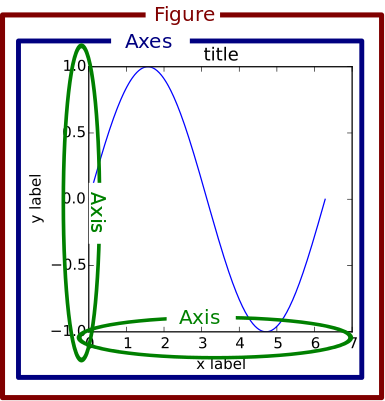
\includegraphics[scale=0.31]{fig_map.png}
\end{center}
\end{column}
\end{columns}

\ \newline
If you are in Jupyter then use \highlt{\texttt{\%matplotlib inline}}
\newline
Most backends support png, pdf, ps, eps and svg.
\newline
The supported file formats depend on the selected backend...
\end{frame}

%%%%%%%%%%%%%%%%%%%%%%%%%%%%%%%%%%%%%%%%%%%%%%%%%%%%%%%%%%%%%%%%%%%%%%%%%%%%%%%%
\begin{frame}[fragile]
\frametitle{Backends}
\begin{center}
  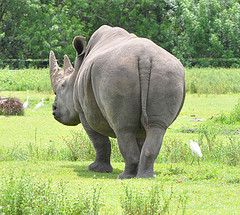
\includegraphics[scale=1.2]{backend.jpg}
\end{center}

\begin{code}
import matplotlib as mpl
mpl.use('PS')
\end{code}

\begin{center}
  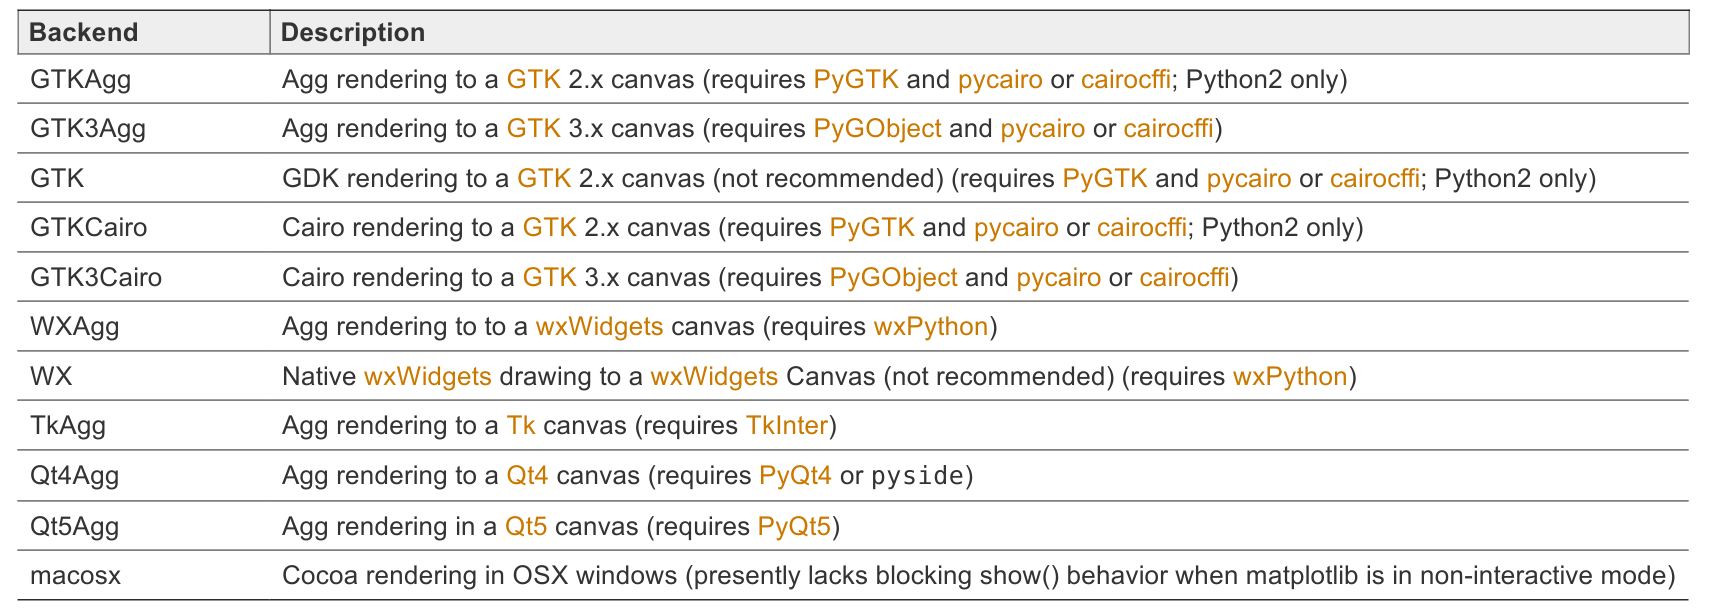
\includegraphics[scale=0.15]{backends-table.png}
\end{center}

\end{frame}

%%%%%%%%%%%%%%%%%%%%%%%%%%%%%%%%%%%%%%%%%%%%%%%%%%%%%%%%%%%%%%%%%%%%%%%%%%%%%%%%
\begin{frame}[fragile]
\frametitle{Start simple and build}

\begin{code}
import matplotlib.pyplot as plt
fig = plt.figure(figsize=(8,4))
ax = fig.add_subplot(111)

ax.set_ylabel('something')
ax.set_title('something')

t = np.arange(0.0, 1.0, 0.01)
s = np.sin(2*np.pi*t)
line, = ax.plot(t, s, color='blue', lw=2)
plt.show()
\end{code}
\end{frame}

%%%%%%%%%%%%%%%%%%%%%%%%%%%%%%%%%%%%%%%%%%%%%%%%%%%%%%%%%%%%%%%%%%%%%%%%%%%%%%%%
\begin{frame}[fragile]
\frametitle{Useful plotting functions}
\footnotesize
\begin{center}
    \begin{table}
        \begin{tabular}{|c|l|}
	\hline
	command                  & description                     \\
	\hline 
	\texttt{plot}            & plot lines and/or markers  \\
	\texttt{bar}             & bar plot                   \\
	\texttt{error bar}       & error bar plot             \\
	\texttt{boxplot}         & boxplot                    \\
	\texttt{histogram}       & histogram                  \\
	\texttt{pie}             & pie charts                 \\ 
	\texttt{imshow}          & heatmaps/images            \\
	\texttt{scatter}         & scatter plots              \\ 
	\hline 
	\end{tabular}
    \end{table}
\end{center}

The \href{http://matplotlib.org/gallery.html}{gallery} will be your new friend
\end{frame}

%%%%%%%%%%%%%%%%%%%%%%%%%%%%%%%%%%%%%%%%%%%%%%%%%%%%%%%%%%%%%%%%%%%%%%%%%%%%%%%%
\begin{frame}[fragile]
\begin{block}{}
 To the Notebooks
\end{block}
\end{frame}

%%%%%%%%%%%%%%%%%%%%%%%%%%%%%%%%%%%%%%%%%%%%%%%%%%%%%%%%%%%%%%%%%%%%%%%%%%%%%%%
\frame{
\begin{block}{Goals}
\begin{enumerate}
 \item Understand how figures, subplots, axes work together in matplotlib, seaborn, and pandas
 \item Use plots and subplots effectively to explore a dataset
 \item Distinguish between different categories on the same plot
 \item Plot inside and outside of ipython notebooks
 \item Understand MPL fundamentals well enough to learn effectively
\end{enumerate}
 \end{block}
}

%%%%%%%%%%%%%%%%%%%%%%%%%%%%%%%%%%%%%%%%%%%%%%%%%%%%%%%%%%%%%%%%%%%%%%%%%%%%%%%
\section{customizing}
\subsection{}

%%%%%%%%%%%%%%%%%%%%%%%%%%%%%%%%%%%%%%%%%%%%%%%%%%%%%%%%%%%%%%%%%%%%%%%%%%%%%%%%
\begin{frame}[fragile]
\frametitle{So much we can do with the axes}
\scriptsize
Plot 1
\begin{code}
ax1 = fig.add_subplot(221)
ax2 = fig.add_subplot(222)
ax3 = fig.add_subplot(222)
ax4 = fig.add_subplot(222)
\end{code}
Plot 2
\begin{code}
ax1 = fig.add_subplot(221)
ax2 = fig.add_subplot(212)
\end{code}
Plot 3 \ \\
\highlt{Hint:} \texttt{add\_axes(left,bottom,width,height}
\begin{code}
ax1 = fig.add_subplot(211)
ax2 = fig.add_axes([0.25,0.1,0.5,0.3])
\end{code}
\end{frame}

%%%%%%%%%%%%%%%%%%%%%%%%%%%%%%%%%%%%%%%%%%%%%%%%%%%%%%%%%%%%%%%%%%%%%%%%%%%%%%%%
\begin{frame}[fragile]
\frametitle{Useful customization functions}
\footnotesize
\begin{center}
    \begin{table}
        \begin{tabular}{|c|l|}
	\hline
	command                      & description                     \\
	\hline
	\texttt{text}            & add text to an axis        \\
	\texttt{table}           & embed a table in the axes  \\
	\texttt{suptitle}        & figure title               \\
	\texttt{ylim/xlim}       & get/set the limits of x and y  \\ 
	\texttt{imshow}          & heatmaps/images            \\
	\texttt{xticks/yticks}   & get/set limits of tick locations  \\
	\texttt{tight\_layout}   & tries to make whitespace look right \\
	\hline
	\end{tabular}
    \end{table}
\end{center}
\end{frame}


%%%%%%%%%%%%%%%%%%%%%%%%%%%%%%%%%%%%%%%%%%%%%%%%%%%%%%%%%%%%%%%%%%%%%%%%%%%%%%%%
\begin{frame}[fragile]
\frametitle{style\_sheets}

\begin{code}
 with plt.style.context('fivethirtyeight'):
    plt.plot(x, np.sin(x) + x + np.random.randn(50))
    plt.plot(x, np.sin(x) + 0.5 * x + np.random.randn(50))
    plt.plot(x, np.sin(x) + 2 * x + np.random.randn(50))
\end{code}

or

\begin{code}
plt.style.use('dark_background')
\end{code}

But be careful with the latter in Jupyter!

\end{frame}

%%%%%%%%%%%%%%%%%%%%%%%%%%%%%%%%%%%%%%%%%%%%%%%%%%%%%%%%%%%%%%%%%%%%%%%%%%%%%%%
\section{higher-level}
\subsection{}
%%%%%%%%%%%%%%%%%%%%%%%%%%%%%%%%%%%%%%%%%%%%%%%%%%%%%%%%%%%%%%%%%%%%%%%%%%%%%%%

\frame{
\frametitle{Higher level interfaces}
\normalsize
\begin{itemize}
 \item \highlt{seaborn} 
 \item \highlt{holoviews}
 \item \highlt{ggplot}
 \end{itemize}
}

%%%%%%%%%%%%%%%%%%%%%%%%%%%%%%%%%%%%%%%%%%%%%%%%%%%%%%%%%%%%%%%%%%%%%%%%%%%%%%%
\frame{
\frametitle{Where do we go from here?}

\begin{block}{}
 \begin{itemize}
  \item 3D plots in MPL
  \item Interactive widgets in MPL
  \item Embedded plots
  \item Image analysis - PIL
  \item Mayavi - 3D data viz
 \end{itemize}
\end{block}
}

\frame{ 
\frametitle{Useful links}
\begin{itemize}
   \item \href{http://matplotlib.org/api/pyplot_summary.html}{list of plotting commands}
   \item \href{http://matplotlib.org/faq/howto_faq.html}{matplotlib howtos}
   \item \href{http://matplotlib.org/users/pyplot_tutorial.html\#pyplot-tutorial}{pylab tutorial}
   \item \href{http://matplotlib.org/users/artists.html\#artist-tutorial}{artist tutorial}
   \item \href{http://matplotlib.org/faq/usage_faq.html}{FAQs}
 \end{itemize}
}


%%%%%%%%%%%%%%%%%%%%%%%%%%%%%%%%%%%%%%%%%%%%%%%%%%%%%%%%%%%%%%%%%%%%%%%%%%%%%%%%%%%%%%%%%%
\section{references}
%%%%%%%%%%%%%%%%%%%%%%%%%%%%%%%%%%%%%%%%%%%%%%%%%%%%%%%%%%%%%%%%%%%%%%%%%%%%%%%%%%%%%%%%%%

\frame[allowframebreaks]{
\frametitle{References}
\tiny
\begin{thebibliography}{9}
\bibliographystyle{apalike}
\setbeamertemplate{bibliography item}[article]
\bibitem{Hunter07}  J.D. Hunter, \emph{Matplotlib: A 2D graphics environment}, Computing In Science \& Engineering \textbf{9(3)} (2007), 90--95.
\end{thebibliography}
\normalsize
}

%%%%%%%%%%%%%%%%%%%%%%%%%%%%%%%%%%%%%%%%%%%%%%%%%%%%%%%%%%%%%%%%%%%%%%%%%%%%%%%
%\frame[allowframebreaks]{  
%\begin{tiny} \bibliography{galvanize-refs.bib}
%\bibliographystyle{apalike}          % Style BST file
%\end{tiny}
%}

\end{document}